\chapter{Software Requirements Specification}
	Das Software Requirements Specification, kurz SRS, ist ein veröffentlichter Standard zur Spezifikation einer Software. Der Inhalt eines SRS ist vom Institute of Electrical and Electronics Engineers im Standard IEEE 830-1998 festgehalten.
	
	Die Aufbau dieses Kapitels entspricht der Struktur, die in dem Standard beschriebenen wird. Einige Kapitel des SRS werden jedoch nicht behandelt, da sie keine Relevanz für NoRPG haben oder an einer anderer Stelle in diesem Dokument auftauchen.
	
\section{Einführung}
	Das erste Kapitel des SRS enthält eine Beschreibung und eine Übersicht über alles, was im SRS enthalten ist.
	
	\subsection{Zweck}
		Das SRS beschreibt den kompletten Projektumfang und die Anforderungen an die Software NoRPG. Es illustriert den Zweck und die vollständige Erklärung für die Entwicklung der Software. Dabei werden unter anderem Systemeinschränkungen, Schnittstellen und Interaktionen mit externen Schnittstellen thematisiert\footnote{vgl. Tripp \cite{srsIEEE}(1998) Seite 3}. 
	
		Die Zielgruppe des SRS sind zunächst alle Personen und Gruppen, die in irgendeiner Verbindung mit NoRPG stehen oder jene, die Interesse an der Umsetzung haben \footnote{vgl. Tripp \cite{rozanski2011}(2011) Seite 6}, den sogenannten Stakeholdern. Zudem dient die Spezifikation zur Kommunikation zwischen den Stakeholdern und den Entwicklern.
		
	\subsection{Umfang}
		Dieses SRS handelt von der in Kapitel 2 beschrieben Software NoRPG. 
		
\section{Allgemeine Beschreibung}
	Im zweiten Kapitel des SRS werden allgemeinen Faktoren, die das Produkt und seine Anforderungen betreffen, beschrieben. Dieses Kapitel bietet einen Überblick über die Systemfunktionalitäten und stellt verschiedene Arten von Stakeholdern und deren Interaktionen mit dem System vor. Dieses Kapitel behandelt jedoch nicht die spezifischen Anforderungen, sondern stellt den Hintergrund für diese Anforderungen dar. 

	\subsection{Produktperspektive}
		Das zu beschreibende vollständige System NoRPG besteht aus mehreren Komponenten, die auf unterschiedlichsten weisen mit den St akeholdern kommunizieren. Daher ist es besonders wichtig, das Produkt in unterschiedlichen Perspektiven mit verwandten und geplanten Produkten zu betrachten. Aufgrund dessen werden die System-, Benutzer-, Hardware- und Softwareschnittstellen von NoRPG betrachtet. Neben den vier genannten Schnittstellentypen gibt es weitere, sind jedoch nicht weiter von Bedeutung.
		
		Folgende Grafik stellt dabei die High-Level-View von NoRPG und seinen Komponenten dar. Dabei sind auch die einzelnen Schnittstellen mit anderen Produkten enthalten. (FEHLT NOCH)
		
		\begin{center}
			\includegraphics[width=10cm]{pics/HighLevelView.png}
			\captionof{figure}{System High-Level-View} 
		\end{center}
		
		Wie aus der Grafik entnommen werden kann, besteht NoRPG aus 3 Kernkomponenten. Zunächst die App, die dem Benutzer als grafische Benutzeroberfläche dient. Dies stellt die Benutzerschnittstelle des Systems dar. Die Benutzerschnittstellen beschreiben die Kommunikation zwischen NoRPG und dem User. Der User kann mit NoRPG nur über die Benutzeroberfläche der App interagieren.
		
		Die zweite Kernkomponenten ist die eingebettete lokale Datenbank. Diese ermöglicht es dem User, das Spiel auch ohne eine aktive Internetverbindung zu spielen.

		Die dritte Kernkomponente ist eine Datenbank auf einem Server, welche in zwei Partitionen unterteilt ist. Die eine Partition ist für die Haltung der Spielerdaten und die zweite Partition für die Spieldaten. Die Datenbanken werden in einem späteren Abschnitt spezifiziert. Die Datenbank auf dem Server ermöglicht das Spielen auf mehreren Geräten, benötigt jedoch eine aktive Internetverbindung. Bei aktiver Internetverbindung wird immer als erstes die Datenbank auf dem Server synchronisiert, da der User auch ohne Internetverbindung weitergespielt hat. Zudem bietet die Speicherung der Daten auf einem Server die Möglichkeit, die Daten zu analysieren.
		
		Bei diesen beiden Komponenten handelt es sich um Softwareschnittstellen. Softwareschnittstellen bilden den Übergang zwischen unterschiedlichen Programmen und ermöglichen dadurch den Android + Google play
	
		Jede Systemschnittstelle beschreibt und identifiziert die Funktionalität der Software, um ... to accomplish the system requirement and the interface description to match the system. Dieses Projekt hat in diesem Stadium nicht vor, mit anderen Systemen zu interagieren. Jedoch ist dies nicht hundertprozentig abstreitbar und wird deswegen hier erwähnt.

		Jede Schnittstelle zwischen NoRPG und Hardwarekomponenten des Systems werden als Hardwareschnittstellen bezeichnet. Dazu gehören auch Konfigurationsmerkmale. Das Smartphone und seine Komponenten ist größte Hardwareschnittstelle. Zum Smartphone gehört das Touchscreen, die Lautsprecher oder der WiFi-Adapter. %wenn Datenbank/Server physikalisch vorhanden, dann kommt das dazu

	\subsection{Produktfunktionen}
		In diesem Unterkapitel werden die wichtigsten Funktionen von NoRPG zusammengefasst.
		
		Ziel von NoRPG: Lernspiele zum Herunterladen in der vorgegebenen Reihenfolge anzeigen.
		
		Spieler kann einmalig bei der Registrierung seinen eigenen Charakter erstellten 
		
		Nach erfolgreicher Anmeldung kann er seinen Charakter durch die Spielwelt steuern, mit Elementen im Spiel interagieren.
		
		\begin{itemize}
			\item{Die Interaktion mit NPC's starten eine Unterhaltung, wodurch der Spieler mehr über das Spiel erfahren kann.}
			\item{Die Interaktion mit einer Verschlossenen Truhe zeigt die Lernspiele, die gespielt werden müssen um die Truhe öffnen zu können.}
			\item{Die Interaktion mit einer freigespielten True, ermöglicht dem Spieler die Truhe zu öffnen.}
			\item{Die Interaktion mit Collectables, die durch das Suchen/Reisen gefunden werden können, sammelt diese.}
			\item{Die Interaktion mit der Umwelt (Tiere, Bäume, etc.) startet keine Aktion.}
		\end{itemize}
		
		Menü mit mehreren Funktionen: Neben kleineren Funktionen wie Spieloptionen gibt es die Möglichkeit den Lernfortschritt zu betrachten, etc.
		
		%Graifk wo die Funktionen in Beziehungen stehen, vielleicht Interaktion bisschen kürzer fassen
	
	\subsection{Benutzermerkmale}
		In diesem Projekt wird zwischen zwei Benutzergruppen unterschieden.
		
		Die erste Benutzergruppe sind die Spieler, die User bzw. die Kinder. Grundsätzlich richtet sich NoRPG an Kinder, die keine Möglichkeit haben eine Schule zu besuchen. Jedoch werden keine Benutzergruppen für diese App ausgeschlossen. Egal ob jung oder alt sowie männlich oder weiblich. %religion, herkunft, ... aufzählen oder to much? :D		
		Der Spieler sollte Erfahrung mit der Verwendung eines Smartphones, insbesondere eines Android-Systems, haben. Dazu zählt die Bedienung der Android-Oberfläche und die des Google Play Stores, da die. Zudem sollte der Spieler die englische Sprache verstehen können, da NoRPG zunächst nur in Englisch erscheinen wird. Jedoch wird das Spiel in jedem Land verfügbar sein, denn bei den vermittelten Standards handelt es sich um international geltende.
		
		Bei der Implementierung ist es wichtig, dass die englischen Texte einfach zu lesen und zu verstehen sind. Denn bei den meisten Benutzern handelt es sich um Kinder zwischen der ersten und fünften Klasse. Zum Voranschreiten ist es notwendig, dass der Spieler den Inhalt von NoRPG versteht. Aus diesem Grund ist eine einfache Sprache ohne Fachjargon notwendig.
		
		Die zweite Benutzergruppe sind die Administratoren.	Administratoren wollen Daten analysieren und daraus Aktionen ableiten. Welche Daten wie gespeichert werden, werden in den spezifischen Anforderungen genauer definiert. 
			
	\subsection{Einschränkungen}
		Bei den Einschränkungen wird zwischen Einschränkungen der Entwickler und Einschränkungen der Spieler unterschieden.
		
		%Einschränkung Entwickler
		Entwickler müssen sich an regulatorische Richtlinien, wie beispielsweise die Datenschutzerklärung von Google oder das IT-Sicherheitsgesetz, halten.
				
		Da NoRPG sich an Kinder in bildungsfernen Ländern richtet, darf NoRPG keine hohen Hardwareressourcen anfordern. Als Maßstab wird das Smartphone Samsung Galaxy S4 genommen %HIER BEGRÜNDUNG WIESO DAS SMARTPHONE und QUELLE. 
		Das Samsung Galaxy S4 kostet 250€\footnote{Stand 04.01.2017 Quelle: sdaqdsa} und hat einen Quadcore?? mit 1,6GHz und 2GB RAM sowie 16GB internen Speicher. Es ist die Android Version 5.0 Lollipop standardmäßig von Samsung installiert.
		
		Schnittstellen anbieten, wenn eine Webapplikation für Administratoren entwickelt wird um Daten besser auszuwerten. Oder Schnittstellen für Spielentwickler. (Bestätigen, dass das Kind den Kurs erfolgreich abgeschlossen hat)
				
		Verfügbar- und Zuverlässigkeit: Spiel muss Offline spiel und -startbar sein. Das Spiel muss sicherstellen, dass ein Kurs vollständig absolviert wird, damit keine verfälschten Daten gesendet werden. 

		Daten der Spieler werden anonymisiert gespeichert um anschließend Analysen zu machen, um rauszufinden in welchen Ländern, Stadtteilen oder Gegenden die meisten Kinder aktiv sind. Daher sollten nur relevante und notwendige Informationen gespeichert werden um diese dann analysieren zu können.
		
		%Einschränkung Spieler
		Internet zum Downloaden von Spielen, von NoRPG, installieren von Updates, Synchronisieren, Registrieren, Einloggen, Ausloggen (da Synchronisiert wird) 
		
		Genügend Speicherplatz, RAM und andere Ressourcen
				
	\subsection{Annahmen und Abhängigkeiten}
		Eine Annahme von NoRPG ist, dass es immer auf Smartphones, die genügend Leistung haben, verwendet wird. Wenn das Telefon nicht über genügend Hardwareressourcen für die Anwendung verfügt, kann es Szenarien geben, in denen die Anwendung nicht wie beabsichtigt oder überhaupt nicht funktioniert.
		
		Eine weitere Annahme ist, dass das Smartphone und dessen Hardware sowie Software funktionieren. Das Smartphone muss sich mit dem Internet verbinden können, wenn der Benutzer sich anmelden möchte oder Lernspiele herunterladen will. Neben einer funktionierenden Internetverbindung sollten andere Hardwareelemente wie die Lautsprecher oder der Touchscreen funktionieren. Das Smartphone muss eine gültige Android Version mit einem Google Konto besitzen.
		
	\subsection{Aufteilung der Anforderungen}
		In dem Fall, dass das Projekt verzögert wird, gibt es einige Anforderungen, die auf die nächste Version der Anwendung übertragen werden könnten.

\section{Spezifische Anforderungen}
	Das letzte Kapitel des SRS dient dazu alle Softwareanforderungen detailliert zu beschreiben. Dies ermöglicht es Designern ein System zu entwickeln, welches allen Anforderungen entspricht, und Testern das System ausreichend zu testen.
	
	Das letzten Kapitel des SRS enthält ausführlich die Anforderungsspezifikation und eine Beschreibung der unterschiedlichen Systemschnittstellen. Es werden verschiedene Spezifikationstechniken verwendet, um die Anforderungen für unterschiedliche Zielgruppen genau festzulegen.
	
	\subsection{Externe Schnittstellen}
		Dieser Abschnitt ist die detaillierte Beschreibung aller Ein- und Ausgänge von NoRPG. Die Beschreibung ergänzt und vervollständigt die Schnittstellenbeschreibung von Kapitel 2.2.1. 
	
	%It should include both content and format as follows:
	%	a) Name;
	%	b) Beschreibung Zweck;
	%	c) Quelle des Inputs und Ziele des Outputs;
	%	d) Gültigkeitsbereich, Genauigkeit + Toleranz;
	%	e) Maßeinheit;
	%	f) Timing;
	%	g) Beziehungne zu anderen In-/Outputs;
	%	h) Screen(Bildschirm)format /-organisation;
	%	i) Fenster(Window)format /-organisation;
	%	j) Datenforrmat;
	%	k) Kommandoformat;
	%	l) End messages.
		
		\subsubsection{Benutzerschnittstellen}
			Die Benutzerschnittstellen, die user interfaces, sind der Punkt, an dem der Benutzer mit der Software interagiert. Zur Beschreibung der Benutzerschnittstellen werden logische Eigenschaften sowie Aspekte zur Optimierung formuliert.
			
			Einem Benutzer, der NoRPG zum ersten Mal startet oder der nicht angemeldet ist, wird der Login-Screen präsentiert. Auf dem Login-Screen hat der Benutzer die Möglichkeit sich mit seinem Benutzernamen und seinem Passwort anzumelden oder sich, falls noch nicht geschehen, bei NoRPG zu registrieren. Das Smartphone muss Quer gehalten werden, da alle Elemente des Bildschirms vertikal angeordnet sind. Diese Eigenschaft trifft auch auf alle anderen Benutzerschnittstellen zu. Das Layout des Login-Screens ist ein Border-Pane, in dem die Bestandteile in einer einzigen Spalte angeordnet sind. Zur Optimierung der Nutzung werden kurze Fehlermeldungen ausgegeben, wenn der Benutzer falsche Login-Daten eingibt.
			\begin{center}
				\includegraphics[width=10cm]{pics/Login_Mockup.png}
				\captionof{figure}{Login-Screen Mockup} 
			\end{center}
			
			Falls sich der Benutzer bei NoRPG registrieren möchte, hat er die Möglichkeit dies in der App zu machen. Dazu klickt der Benutzer im Login-Screen auf den Register-Button. Anschließend öffnet sich der Register-Screen. Die Elemente sind im Tabellen Layout angeordnet, wodurch der Benutzer weiß, welche Daten in welches Feld eingetragen werden müssen. Die Registrierung ist notwendig, damit der Spielstand, somit der Fortschritt in einer Relation mit dem Benutzer steht. Zur weiteren Optimierung werden kurze Fehlermeldungen ausgegeben, damit ich der Benutzer weiß, in welchem Feld ein Fehler ist.
			
			\begin{center}
				\includegraphics[width=10cm]{pics/Register_Mockup.png}
				\captionof{figure}{Register-Screen Mockup} 
			\end{center}
			
			Nach der Registrierung kann der Spieler einmalig seinen Charakter für den angelegten Account erstellen. Dazu bestimmt der Benutzer den Namen, das Geschlecht und das Aussehen des Charakters.
			
			\begin{center}
				\includegraphics[width=10cm]{pics/Register_Mockup.png}
				\captionof{figure}{Register-Screen Mockup} 
			\end{center}
			
			NoRPG startet, nachdem alles geladen wurde und der Benutzer angemeldet ist. Das Spiele-Screen besteht aus der Spielewelt (Grafik) und dem Head-Up Display, kurz HUD. Das HUD ist eine Methode, mit der Informationen visuell als Teil der Benutzeroberfläche eines Spiels vermittelt werden. Während die Informationen, die auf dem HUD angezeigt werden, stark vom Spiel abhängen, gibt es viele Eigenschaften, die Spieler über viele Spiele erkennen. Die meisten von ihnen sind statisch auf dem Bildschirm, so dass sie während des Spiels sichtbar bleiben. 
			
			\begin{center}
				\includegraphics[width=11cm]{pics/HUD_Mockup.png}
				\captionof{figure}{HUD Mockup} 
			\end{center}
			
			Das Mockup 3 enthält alle direkt sichtbaren HUD Elemente, die während des Spieles aktiv sind. Die Elemente sind an die Ecken gebunden, so befindeen sich beispielsweise die Pfeiltasten zur Bewegung des Charakters in der linken unteren Ecke des Bildschirms (siehe Graifk). Es sind so wenig Elemente wie möglich auf dem Bildschirm angeordnet und die verwendeten Symbole sind aus anderen bekannten Spielen und Konsolen übernommen und sind quasi ein Standard. Durch diese bekannte Anordnung der Elemente kann der User Informationen schneller verstehen und schneller reagieren. %vllt bisschen noch was zu dieser Anordnung labern
			
			Das Menü, welches sich in der oberen linken Ecke befindet, kann geöffnet werden. Dadurch wird das laufende Spiel pausiert und es werden weitere Optionen bzw. Interaktionen mit dem Spiel möglich. Diese HUD Elemente werden nur dann sichtbar, wenn der Spieler das Menü öffnet. Dadurch rückt das Spiel und die anderen Elemente in den Hintergrund. Das bedeutet nicht, dass die Elemente ausgeblendet werden, sondern dass der Benutzer diese Elemente nicht benutzen kann solange das Menü offen ist.
			
			\begin{center}
				\includegraphics[width=11cm]{pics/HUD_Mockup.png}
				\captionof{figure}{HUD offenes Menü Mockup} 
			\end{center}
			
			Einige der Menü-Elemente öffnen wiederum einen anderen Screen. Diese werden dann über das aktuelle Spiel geöffnet. Das Spiel befindet sich im Hintergrund und kann nicht gesehen bzw. angeklickt werden. Der neu geöffnete Screen muss erst geschlossen werden um das Spiel fortsetzen zu können. Ein Beispiel dafür ist der Fortschritt-Screen. Hier kann der Benutzer seinen Lern- bzw. Spielfortschritt betrachten.
			
			\begin{center}
				\includegraphics[width=10cm]{pics/Fortschritt_Mockup.png}
				\captionof{figure}{Fortschritt-Screen Mockup} 
			\end{center}
			
			Die Auflistung aller Screens würde den Rahmen dieser Arbeit überschreiten. Daher befinden sich die Mockups für die restlichen Screens im Anhang.
						
			%logische Eigenschaften:  required screen formats, page or window layouts, content of any reports or menus, or availability of programmable function keys
			
			%Aspekte Optimierung: comprise a list of do's and don'ts on how the system will appear to the user: long or short error messages
		
		\subsubsection{Hardwareschnittstellen}
			Die Hardwareschnittstellen spezifiziert die logischen Eigenschaften jeder Schnittstelle zwischen NoRPG und den Hardwarekomponenten des Systems.
			
			NoRPG besitzt keine direkten Hardwareschnittstellen: Verbunden mit Lautsprechern für Soundausgaben, Touchscreen für Eingaben/Interaktionen, WLAN für die Verbindung mit dem Server/Synchronisierung, Verbindung zum Datenbank Server
			
		\subsubsection{Softwareschnittstellen}
			This should specify the use of other required software products and interfaces with other application systems 
			
			Data mangement system, Android OS

	\subsection{Funktionale Anforderungen}
		Use Cases dokumentieren Funktionalitäten eines Systems auf Basis von einfachen Modellen. In einem Use Case wird das nach außen sichtbare Verhalten eines Systems aus der Sicht der Nutzer beschrieben. Ein Nutzer kann hierbei eine Person, eine Rolle oder ein anderes System sein. Dieser Nutzer tritt als Akteur mit dem System in Interaktion, um ein bestimmtes Ziel zu erreichen. %quelle
		
		Use Cases verwenden Activity UML um anzuzeigen, wie der Benutzer vorgehen muss. Ein Aktivitätsdiagramm ist ein Verhaltensdiagramm der Unified Modeling Language (UML) und stellt die Vernetuzung von elementaren Aktionen und deren Verbindungen mit Kontroll- und Datenflüssen grafisch dar.
	
		\begin{center}
			\includegraphics[width=10cm]{pics/OUCD.pdf}
			\captionof{figure}{Overall Use Case Diagramm} 
		\end{center}
		
		Das abgebildete System stellt die zu entwickelnde App für die User dar. Die App stellt die Graphische Oberfläche und somit die beschrieben Benutzerschnittstellen dar. Es sind nur die Funktionalitäten enthalten, die der Benutzer ausführen kann, also jene die über die Benutzerschnittstellen angesprochen werden können. Use Cases wie Login oder Registrierung sind im Overall Use Case Diagramm nicht enthalten, da diese im Vergleich zu anderen Use Cases primitiv sind. 
	
		\subsubsection{Create character}
			Dieser Use Case beschreibt den Anwendungsfall, dass der Benutzer seinen Charakter erstellen möchte. Dieser Use Case wird pro Account genau einmal nach der Registrierung ausgeführt und zählt noch zum Prozess der Registrierung.
			
			Nach erfolgreicher Registrierung kann der Spieler seinen Charakter erstellen. Der User kann seinem Charakter einen Namen geben, das Geschlecht auswählen und anschließend das Aussehen bestimmen. Anschließend wird dem User der Hinweis angezeigt, dass es sich um eine einmalige Aktion handelt. Nachdem diese bestätigt wurde, wird der Charakter erstellt und gespeichert.
				
			\begin{center}
				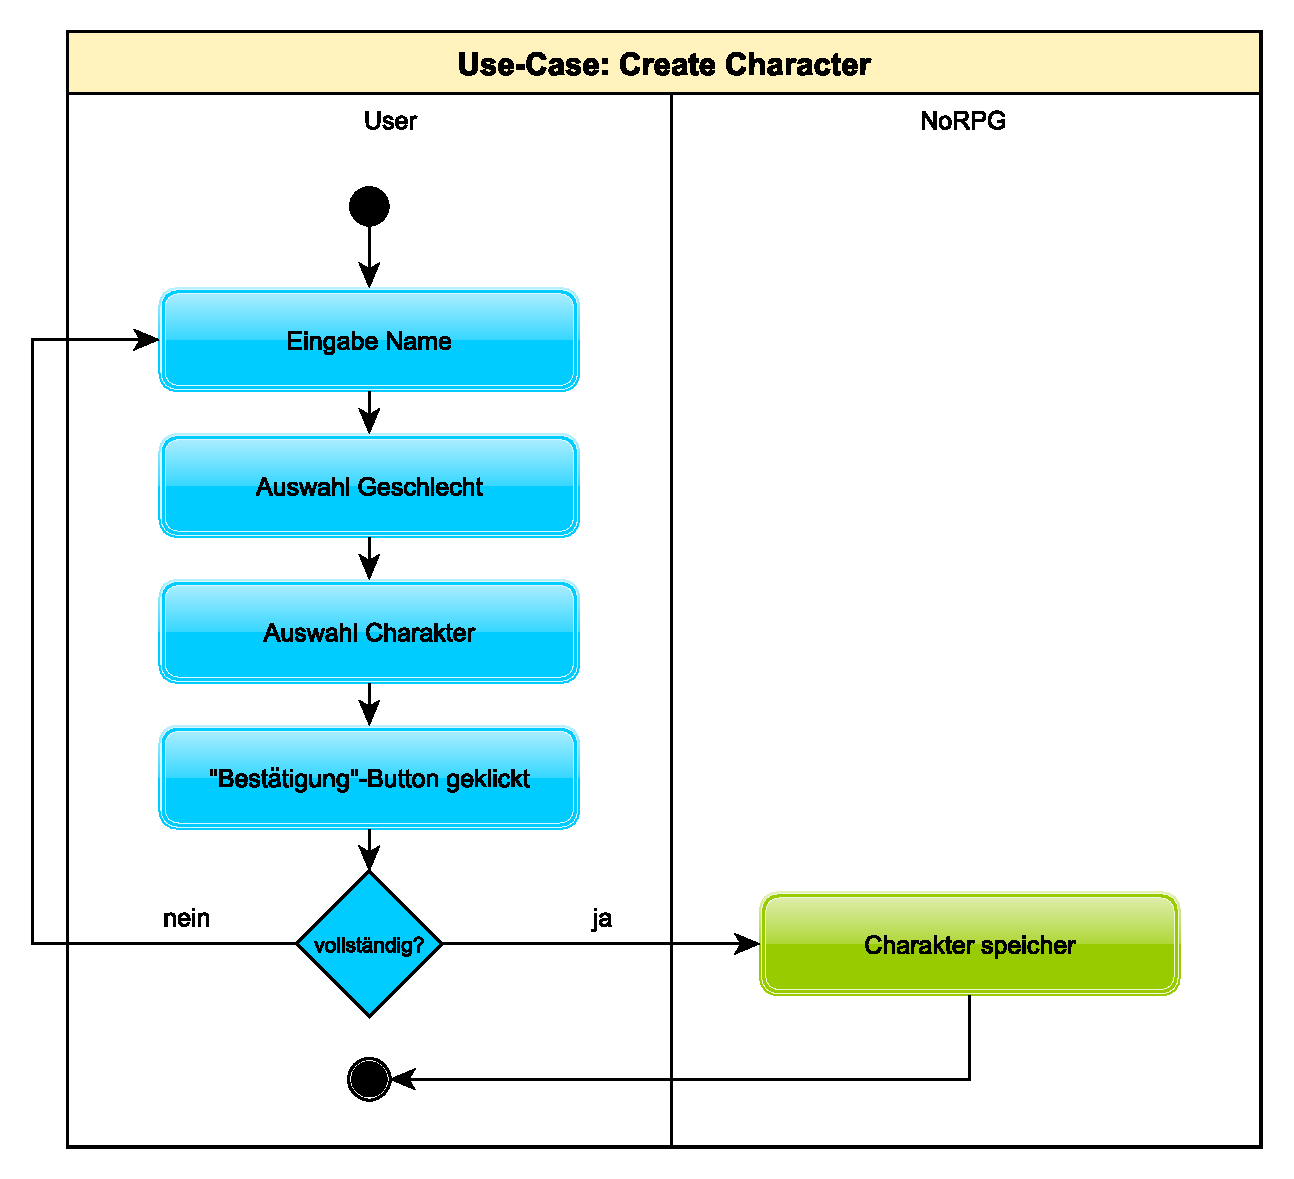
\includegraphics[width=10cm]{pics/CreateCharacter.pdf}
				\captionof{figure}{Create Character Activity UML} 
			\end{center}
	
			Bevor jedoch dieser Use Case ausgeführt werden kann, muss die Registrierung vollständig und erfolgreich abgeschlossen werden. Die Registrierung ist erfolgreich, wenn alle benötigte Daten eingetragen wurden und der Account noch nicht existiert. Für den gesamten Registrierungsprozess wird eine aktive Internetverbindung benötigt.
			
			Nach erfolgreicher Erstellung des Charakters, wird dieser in die Datenbank gespeichert und der User kann sich nun anmelden und in die Rolle seines Charakters schlüpfen.
			
		\subsubsection{Open map}
			Dieser Use Case beschreibt den Anwendungsfall, dass der Benutzer die Karte öffnet. Die Karte dient zur Orientierung der Welt und beinhaltet Symbole etc. um herauszufinden was so ist
			
			Ereignisablauf:	Benutzer öffnet Menü und klickt auf "Map" ...
	
			Vorbedingungen: Menü offen, Benutzer befindet sich nicht in einer NPC Interaktion
			
			Nachbedingungen: Eine Karte von der aktuellen Welt wird geöffnet
	
		\subsubsection{Show games}
			Dieser Use Case beschreibt den Anwendungsfall: Liste der gespielten und heruntergeladneen Spiele wird angezeigt. Zuordnung zu den Standards. Aus NoRPG das Spiel starten können.
			
			Ereignisablauf: Benuter öffnet Menü und klickt auf "Games" ...

			Vorbedingungen: Menü offen, Benutzer befindet sich nicht in einer NPC interaktion
			
			Nachbedingungen: Eine Liste wird angezeigt
	
		\subsubsection{View progress}
			Dieser Use Case beschreibt den Anwendungsfall, dass der Benutzer 
			
			Ereignisablauf
	
			Vorbedingungen
			
			Nachbedingungen
	
		\subsubsection{Settings}
			Dieser Use Case beschreibt den Anwendungsfall, dass der Benutzer 
			
			Ereignisablauf
	
			Vorbedingungen
			
			{Nachbedingungen
	
		\subsubsection{Synchronize}
			Dieser Use Case beschreibt den Anwendungsfall, dass der Benutzer 
			
			Ereignisablauf
	
			Vorbedingungen
			
			Nachbedingungen
	
		\subsubsection{Save local}
			Dieser Use Case beschreibt den Anwendungsfall, dass der Benutzer 
			
			Ereignisablauf
	
			Vorbedingungen
			
			Nachbedingungen
		
		\subsubsection{Character control}
			Dieser Use Case beschreibt den Anwendungsfall: Benutzer interaktionen, wie Bewegen oder Bestätigen.
			
			Ereignisablauf
			
			Vorbedingungen: Spieler befindet sich im Spiel (nicht loading screen und menü ist geschlossen)
			
			Nachbedingungen: Charakter bewegt sich, bestätigt oder lehnt ab
	
		\subsubsection{game interaction}
			Dieser Use Case beschreibt den Anwendungsfall, dass der Benutzer sich in einer Interaktion mit einem NPC befindet. NPC bedeutet Non-Player Charakter und stellt die programmierten Charaktere dar (Unterhaltungen mit NPC, Storytelling)
			
			Ereignisablauf
			
			Vorbedingungen: Spieler befindet sich im Spiel (nicht loading screen und menü ist geschlossen)
			
			Nachbedingungen: Charakter bewegt sich, bestätigt oder lehnt ab
	
	\subsection{Performanz Anforderungen}
		This subsection should specify both the static and the dynamic numerical requirements placed on the software or on human interaction with the software as a whole. Static numerical requirements may include the following
		
		The number of terminals to be supported, The number of simultaneous users to be supported, Amount and type of information to be handled
		
	\subsection{Datenbank Anforderungen}
		This should specify the logical requirements for any information that is to be placed into a database. This may include the following:
		
		Types of information used by various functions
		
		Frequency of use
		
		Accessing capabilities
		
		Data entities and their relationships
		
		Integrity constraints
		
		Data retention requirements.
	
	\subsection{Entwurfsbeschränkungen}
		This should specify design constraints that can be imposed by other standards, hardware limitations, etc.
		
		Standards compliance: This subsection should specify the requirements derived from existing standards or regulations. They may include the following: 
		
		Report format, Data naming, Accounting procedures and Audit tracing.
	
	\subsection{Benuzterfreundlichkeit}

	\subsection{Zuverlässigkeit}
		This should specify the factors required to establish the required reliability of the software system at time of delivery.
	
	\subsection{Verfügbarkeit}
		This should specify the factors required to guarantee a defined availability level for the entire system such as checkpoint, recovery, and restart. 
	
	\subsection{Sicherheit}
		This should specify the factors that protect the software from accidental or malicious access, use, modification, destruction, or disclosure. Specific requirements in this area could include the need to
		
		Utilize certain cryptographical techniques; 
		
		Keep specific log or history data sets;
		
		Assign certain functions to different modules;
		
		Restrict communications between some areas of the program;
		
		Check data integrity for critical variables.
	
	\subsection{Wartbarkeit}
		This should specify attributes of software that relate to the ease of maintenance of the software itself. There may be some requirement for certain modularity, interfaces, complexity, etc. Requirements should not be placed here just because they are thought to be good design practices.
	
	\subsection{Portabilität}
		This should specify attributes of software that relate to the ease of porting the software to other host machines and/or operating systems. This may include the following:
		
		Percentage of components with host-dependent code;
		
		Percentage of code that is host dependent;
		
		Use of a proven portable language; 
		
		Use of a particular compiler or language subset;
		
		Use of a particular operating system.
